\newcommand{\upcite}[1]{\textsuperscript{\textsuperscript{\cite{#1}}}}
\chapter*{\zjutitlec 中期报告}

\section{项目背景}
原始神经元图像信息的神经元追踪和数字重建是神经科学界热门方向。神经元的形态反应出它的功能,相同功能的神经元通常具有类似的功能。神经科学家通过结构脑图谱的重建,可以反推大脑是如何运作,对理解智慧的产生有重要的帮助。Cannon RC 等人在海马神经重建上做出的工作\upcite{Cannon1998An},Feng L 等人使用 mGRASP 在鼠类大脑上进行的重建工作\upcite{Druckmann2014Structured}均取得了出色的进展。

由于神经元拓扑结构的复杂性,在一些自动化重建结果的细节上仍然需要研究人员对数字重建的结果进行人工纠正和修改,以确保数字重建工作的准确性。另外研究人员需要对数字重建结果进行编辑,比如添加或删除一些网络分支等。为了便于研究人员编辑数字重建的结果,根据“所见即所得”的原则,设计出了 SWC 格式\upcite{Peng2011Proof}。SWC 框架有以下特征: 清楚的 SWC 结构以及原始数据参考的可视化,明确定义的可操作单元,以及将用户输入和编辑操作直观地对应起来。在 SWC 格式的基础上,研究人员可以方便、直观地纠正自动化数字重建结果的错误,添加新的分支或删除已有分支。Feng,Linqing, Zhao Ting, Kim Jinhyun 等人\upcite{Feng2014neuTube}充分充分发挥了 SWC 格式高效,精确的优点,提供了同时在 2D 和 3D 模式下查看,编辑神经元结构的功能。

由于 neuTube 是运行在单机的软件,无法满足多用户协同编辑修改的需求,也不利于结构脑图谱的交流。随着计算机性能和网络速度的提升,在线实时编辑神经元网络结构成为了可能。在此背景下,我们希望设计并实现一个在线多用户的神经元网络结构编辑分享平台,利用互联网便于数据共享的特点,帮助神经学研究人员便捷地进行异地,多用户协同编辑神经元网络结构,并能分享结构脑图谱,共同探索神经元结构下的奥秘。

\section{整体架构}
项目整体结构如图 \ref{server} 所示,共分为神经信息数据库,用户信息数据库以及网络服务器三部分组成。
\begin{figure}
\centering
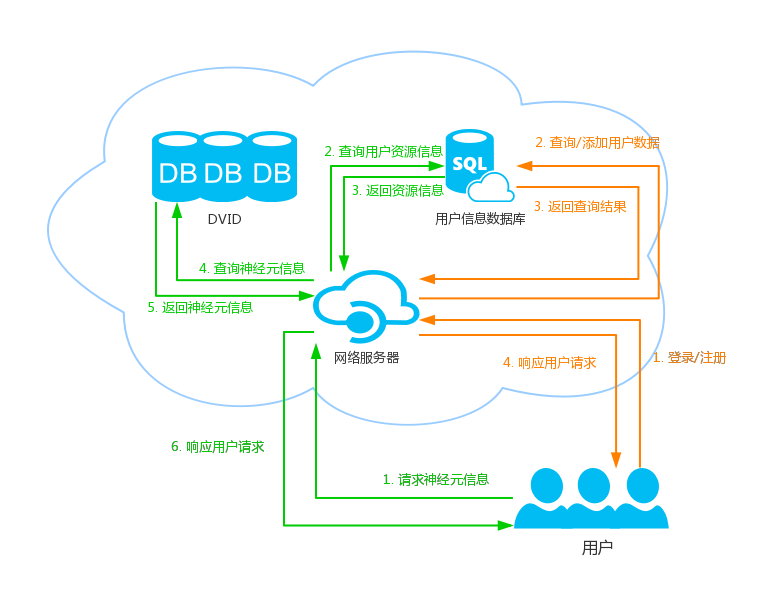
\includegraphics[width=108mm]{images/server}
\caption{项目整体架构}
\label{server}
\end{figure}

\subsection{神经信息数据库}

\bibliographystyle{data/gbt7714-2005}
{
\renewcommand{\chapter}[2]{\section*{#2}\addcontentsline{toc}{section}{#2}}
\bibliography{data/zhongqi}
}